\chapter{Introduction}
\section{Ist-Situation}
Im Unternehmen “Augenoptik Aigner” sind zur Zeit nur wenige Rechner im Einsatz, welche alle mit dem Betriebssystem “Windows 95” funktionieren. Auf diesen existiert ein Dos-Programm welches Kunden,  Aufträge, Lieferanten und lagernde Produkte  verwaltet. Weil mehrere Rechner im Einsatz sind, muss die aktuelle Version des Programms immer auf den Rechner kopiert werden, auf dem man dann gerne arbeiten würde. Dies ist natürlich sehr umständlich und zeitaufwendig, weshalb es Zeit wird, alle Rechner auf ein aktuelles Betriebssystem zu aktualisieren und eine zentrale Datenbank einzurichten, damit alle Rechner immer synchronisiert sind.

Die Website des Unternehmens Augenoptik Aigner ist aktuell weder responsive noch ist sie visuell ansprechend außerdem ist sie in der Funktionalität beschränkt. Die einzigen Funktionen die man hat sind allgemeine Daten anzusehen, wie die Geschäftszeiten, den Standort des Unternehmens, ein Impressum und man kann den Verkäufer noch mittels eines Formulars kontaktieren. 

\section{Zielsetzung}


\section{Overview}
Details of the diploma thesis have to be aligned between student and supervisor. This should be a basic structure to facilitate the first steps when students start to write their theses.

Never forget to add some illustrative images. Images must not be messed up with your normal text. They are encapsulated in floating bodies and referenced in your text. An example can be seen in figure~\ref{fig:sample}. As you can see, figures are placed by default on top of the page nearby the place where they are referenced the first time. Furthermore you can see that a list of figures is maintained automatically which can be included easily by typing the command \verb1\listoffigures1 into your document.

\begin{figure}
\begin{center}
	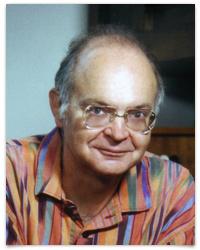
\includegraphics[scale=.5]{images/don_knuth.jpg}
\end{center}
	\caption{Don Knuth, the inventor of \TeX}
	\label{fig:sample}
\end{figure}

\section{Basic Terminology}
As usual the very basic terminology is briefly explained here. Most probably the explanations here only scratch a surface level. More detailed explanations of terminology goes into chapter~\ref{cha:theoretical-background}.

\section{Related Work and Projects}
Here a survey of other work in and around the area of the thesis is given. The reader shall see that the authors of the thesis know their field well and understand the developments there. Furthermore here is a good place to show what relevance the thesis in its field has.

\section{Structure of the Thesis}
Finally the reader is given a brief description what (s)he can expect in the thesis. Each chapter is introduced with a paragraph roughly describing its content.~\ref{cha:theoretical-background} 
Online Referenz: \cite{wikipedia_.net_2017}
\end{comment}